\chapter{观测器}
\label{chap:chapter03}
\section{移动平均滤波}
简单移动平均(英语:simple moving average,SMA)是某变数之前$n$个数值的未作加权算术平均
\begin{equation}
  \text{SMA}=\frac{p_1+p_2+\cdots + p_n}{n}
\end{equation}
当计算连续的数值,一个新的数值加入,同时一个旧数值剔出,所以无需每次都重新逐个数值加起来:
\begin{equation}
  \text{SMA}_{t1,n}=  \text{SMA}_{t0,n}-\frac{p_1}{n} +\frac{p_{n+1}}{n}
\end{equation}
然而,移动平均滤波的结果存在时滞,当$n$较大时,滤波器产生的结果将不可靠。

\section{卡尔曼滤波}
\subsection{概述}

卡尔曼滤波(Kalman filter)是一种高效率的递归滤波器(自回归滤波器),
它能够从一系列的不完全及包含噪声的测量中,估计动态系统的状态。
卡尔曼滤波会根据各测量量在不同时间下的值,考虑各时间下的联合分布,
再产生对未知变数的估计,因此会比只以单一测量量为基础的估计方式要准。

卡尔曼滤波建立在线性代数和隐马尔可夫模型(hidden Markov model)上。
其基本动态系统可以用一个马尔可夫链表示,该马尔可夫链建立在一个被高斯噪声
(即正态分布的噪声)干扰的线性算子上的。系统的状态可以用一个元素为实数的向量表示。
随着离散时间的每一个增加,这个线性算子就会作用在当前状态上,产生一个新的状态,
并也会带入一些噪声,同时系统的一些已知的控制器的控制信息也会被加入。
同时,另一个受噪声干扰的线性算子产生出这些隐含状态的可见输出。

\subsection{模型}
如图\ref{fig:Basic_concept_of_Kalman_filtering}所示,
为了从一系列有噪声的观察数据中用卡尔曼滤波器估计出被观察过程的内部状态,
必须把这个过程在卡尔曼滤波的框架下建立模型。也就是说对于每一步$k$,
定义矩阵$\bm{F}_k, \bm{H}_k, \bm{Q}_k, \bm{R}_k$,有时也需要定义$\bm{B}_k$,如下。

卡尔曼滤波模型假设$k$时刻的真实状态是从$(k-1)$时刻的状态演化而来,符合下式:
\begin{equation}
  \bm{x}_k=\bm{F}_k \bm{x}_{k-1} + \bm{B}_k \bm{u}_{k} + \bm{w}_k
\end{equation}

其中
\begin{itemize}
  \item $\bm{F}_k$是作用在$\bm{x}_{k-1}$上的状态变换模型(/矩阵/矢量)。
  \item $\bm{B}_k$是作用在控制器向量$\bm{u}_k$上的输入-控制模型。
  \item $\bm{w}_k$是过程噪声,并假定其符合均值为零,协方差矩阵为$\bm{Q}_k$的多元正态分布。
  \item $\bm{w}_{k} \sim N(0 \, , \, \bm{Q}_k)$
\end{itemize}

时刻$k$,对真实状态$\bm{x}_k$的一个测量$\bm{z}_k$满足下式:
\begin{equation}
  \bm{z}_k=\bm{H}_k \bm{x}_k + \bm{v}_k
\end{equation}
其中$\bm{H}_k$是观测模型,它把真实状态空间映射成观测空间,$\bm{v}_k$是观测噪声,
其均值为零,协方差矩阵为$\bm{R}_k$,
且服从正态分布$\bm{v}_{k} \sim N(0 \, , \, \bm{R}_k)$。
初始状态以及每一时刻的噪声${\bm{x}_0, \bm{w}_1, \cdots ,
\bm{w}_k, \bm{v}_1, \cdots \bm{v}_k}$都认为是互相独立的。

实际上,很多真实世界的动态系统都并不确切的符合这个模型;
但是由于卡尔曼滤波器被设计在有噪声的情况下工作,
一个近似的符合已经可以使这个滤波器非常有用了
\begin{figure}[!htp]
  \centering
  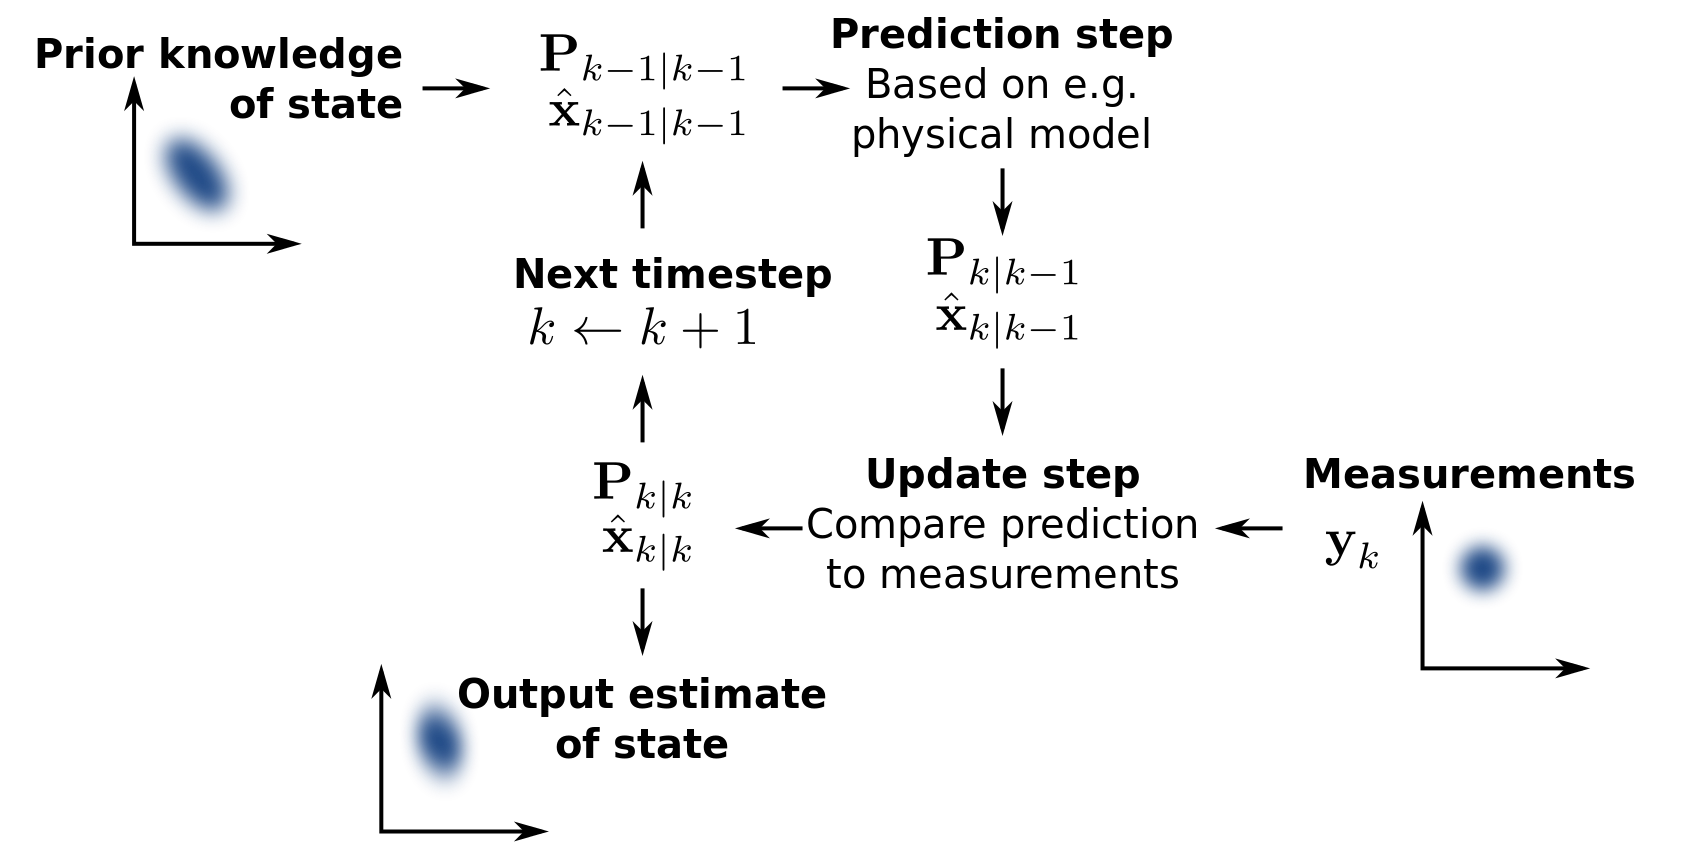
\includegraphics[width=15cm]{chapter03/Basic_concept_of_Kalman_filtering.png}
  \bicaption[卡尔曼滤波的示意图(来自维基百科)]
    {卡尔曼滤波的示意图}
    {The Kalman filter keeps track of the estimated state of the system 
    and the variance or uncertainty of the estimate. 
    The estimate is updated using a state transition model and measurements. 
    $\hat{\bm{x}}_{k \mid k-1}$ denotes the estimate of the system's state 
    at time step $k$ before the $k$-th measurement $\bm{y}_k$ has been 
    taken into account;
    $\bm{P}_{k\mid k-1}$ is the corresponding uncertainty.}
  \label{fig:Basic_concept_of_Kalman_filtering}
\end{figure}

\subsection{算法}
尔曼滤波是一种递归的估计,即只要获知上一时刻状态的估计值以及当前状态的观测值就
可以计算出当前状态的估计值,因此不需要记录观测或者估计的历史信息。
卡尔曼滤波器与大多数滤波器不同之处,在于它是一种纯粹的时域滤波器,
它不需要像低通滤波器等频域滤波器那样,需要在频域设计再转换到时域实现。

卡尔曼滤波器的状态由以下两个变量表示:
\begin{itemize}
  \item $\hat{\bm{x}}_{k | k}$, 在时刻$k$的状态的估计;
  \item $\bm{P}_{k|k}$,后验估计误差协方差矩阵,度量估计值的精确程度。
\end{itemize}

卡尔曼滤波器的操作包括两个阶段:\textbf{预测}与\textbf{更新}。在预测阶段,
滤波器使用上一状态的估计,做出对当前状态的估计。在更新阶段,
滤波器利用对当前状态的观测值优化在预测阶段获得的预测值,以获得一个更精确的新估计值。
\subsubsection{预测}
\begin{equation}
  \begin{aligned}
    &\hat{\bm{x}}_{k|k-1}=\bm{F}_k \hat{\bm{x}}_{k-1 | k-1} + \bm{B}_k \bm{u}_{k} \text{(预测状态)} \\
    &\bm{P}_{k|k-1}=\bm{F}_k \bm{P}_{k-1|k-1} \bm{F}_k^T + \bm{Q}_k
    \text{(预测估计协方差矩阵)}
  \end{aligned}
\end{equation}

\subsubsection{更新}
首先要算出以下三个量:
\begin{equation}
  \begin{aligned}
    &\tilde{\bm{y}}_k = \bm{z}_k - \bm{H}_k \hat{\bm{x}}_{k|k-1}
     \text{(测量余量,measurement residual)} \\
    &\bm{S}_{k}=\bm{H}_k \bm{P}_{k|k-1} \bm{H}_k^T + \bm{R}_k
    \text{(测量余量协方差)} \\
    &\bm{K}_k = \bm{P}_{k|k-1} \bm{H}_k^T \bm{S}_{k}^{-1}
    \text{(最优卡尔曼增益)}
  \end{aligned}
\end{equation}

然后用它们来更新滤波器变量$\bm{x}$与$\bm{P}$:
\begin{equation}
  \begin{aligned}
    &\hat{\bm{x}}_{k|k} = \hat{\bm{x}}_{k|k-1} + \bm{K}_k \tilde{\bm{y}}_k
     \text{(更新的状态估计)} \\
    &\bm{P}_{k|k} =(\bm{I}-  \bm{K}_k \bm{H}_k) \bm{P}_{k|k-1}
    \text{(更新的协方差估计)}
  \end{aligned}
\end{equation}

\subsubsection{不变}
如果模型准确,而且$\hat{\bm{x}}_{0|0}$与$\bm{P}_{0|0}$的值准确的反映了最初状态的分布,
那么以下不变量就保持不变:所有估计的误差均值为零。
\begin{itemize}
  \item $\mathbb{E}[\bm{x}_k - \hat{\bm{x}}_{k|k}] =
      \mathbb{E}[\bm{x}_k - \hat{\bm{x}}_{k|k-1}] = 0$
  \item  $\mathbb{E}[\tilde{\bm{y}}_k]=0$
  \item $\bm{P}_{k|k}= cov(\bm{x}_k - \hat{\bm{x}}_{k|k})$
  \item $\bm{P}_{k|k-1}= cov(\bm{x}_k - \hat{\bm{x}}_{k|k-1})$
  \item $\bm{S}_k = cov(\tilde{\bm{y}}_k)$
\end{itemize}
其中,$\mathbb{E}[a]$表示$a$的期望值,$cov(\bm{a})=\mathbb{E}[\bm{a} \bm{a}^T]$

\subsection{经验}
卡尔曼滤波器中,Q代表Process Noise Covariance Matrix, R代表Measurement Noise
Covariance Matrix; R越小, estimation的结果更"信任"测量值,反之,Q越小,
estimation的结果更"信任"预测值。


\section{GPS天线修正}
由于GPS天线安装的位置不在船体重心处,我们需要对GPS测量结果作修正处理,才能得到重心处的运动。
